\onslide<1->{
   	\tikzstyle{vertex2} = [opacity = 0]
   	\tikzstyle{vertex3} = [opacity = 0]
    \tikzstyle{vertex4} = [opacity = 0]
   	\tikzstyle{vertex5} = [opacity = 0]
    \tikzstyle{vertex9} = [opacity = 0]
    \tikzstyle{vertex11} = [opacity = 0]
}
\only<2->{\tikzstyle{vertex2} = [opacity = 1]}
\only<3->{\tikzstyle{vertex3} = [opacity = 1]}
\only<4->{\tikzstyle{vertex4} = [opacity = 1]}
\only<5->{
  	\tikzstyle{vertex5} = [opacity = 1]
    \tikzstyle{vertex9} = [opacity = 1]
}

\tikzstyle{end} = [circle, minimum size = 0.6cm, draw = black, inner sep = 0.1pt]
            
\tikzstyle{level 1} = [draw = black, level distance = 1.5cm, sibling distance = 5cm]
\tikzstyle{level 2} = [sibling distance = 2cm]
    
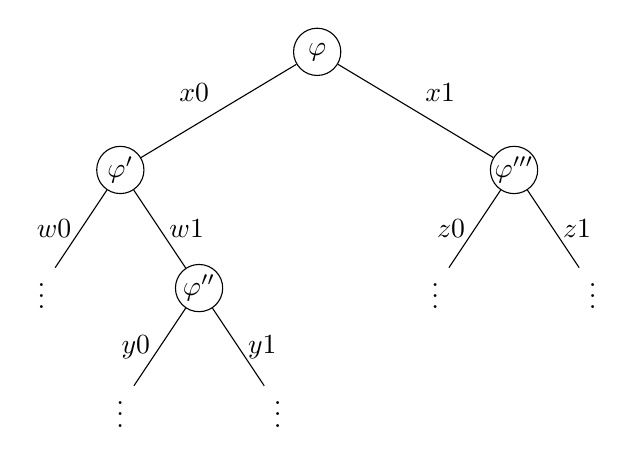
\begin{tikzpicture}[label distance=8mm]
	\node [end] (z){$\varphi$}
		child [vertex2] {
    		node [end] (b) {$\varphi'$}
			child [vertex3]{
	           	node {$\vdots$}
                edge from parent
	  	        node[left] {$w \coloneqq 0$}
            }
		    child [vertex4]{
            	node[end] {$\varphi''$}
            	child [vertex4]{
            	   	node {$\vdots$}
            		edge from parent
	  	        	node[left] {$y \coloneqq 0$}
                }
                child [vertex4]{
            	   	node {$\vdots$}
            		edge from parent
	  	        	node[right] {$y \coloneqq 1$}
            	}
                edge from parent
	   	        node[right] {$w \coloneqq 1$}
            }
           	edge from parent
            node[above left] {$x \coloneqq 0$}
        }
        child [vertex5] {
        	node [end] (c) {$\varphi'''$}
           	child [vertex9]{
               	node {$\vdots$}
                edge from parent
	            node[left] {$z \coloneqq 0$}
            }
		    child [vertex9]{
               	node {$\vdots$}
                edge from parent
	            node[right] {$z \coloneqq 1$}
            }
            edge from parent
	   	    node[above right] {$x \coloneqq 1$}
        };
\end{tikzpicture}